% SEC 2.1
\section{Matrix Operations}
\name

Use the following matrices for the problems on this page.
\begin{align*}
A &= \begin{bmatrix}3&0&-2\\4&-5&3\end{bmatrix} &
B &= \begin{bmatrix}7&-4&2\\2&-3&-2\end{bmatrix} &
C &= \begin{bmatrix}2&3\\-3&2\end{bmatrix} &
D &= \begin{bmatrix}3&6\\-2&3\end{bmatrix} &
E &= \begin{bmatrix}-6\\3\end{bmatrix}
\end{align*}

\begin{exercise} % 2.1.2
	Compute the matrix sum or explain why the expression is undefined.
	\begin{multicols}{2}
		\begin{enumerate}[(a)]
			\item $A+2B$
			\item $4C-2E$
		\end{enumerate}
	\end{multicols}
\end{exercise}
\vfill


\begin{exercise} % 2.1.2
	Compute the matrix product or explain why the expression is undefined.
	\begin{multicols}{2}
		\begin{enumerate}[(a)]
			\item $EB$
			\item $DB$
		\end{enumerate}
	\end{multicols}
\end{exercise}
\vfill


\newpage


\begin{boxme}
	If $A$ is an $m\times n$ matrix and $B=\begin{bmatrix}\vect{b}_1&\vect{b}_2&\cdots&\vect{b}_p\end{bmatrix}$ is an $n\times p$ matrix, then the product $AB$ is the $m\times p$ matrix
	$$ AB = \begin{bmatrix}A\vect{b}_1&A\vect{b}_2&\cdots&A\vect{b}_p\end{bmatrix}. $$
	In other words, each column of $AB$ is a linear combination of the columns of $A$ using the entries of the corresponding columns of $B$ as weights.
\end{boxme}
\begin{exercise} % 2.1.5
	Let $A$ and $B$ be as below. Denote the first and second columns of $B$ by $\vect{b}_1$ and $\vect{b}_2$, respectively.
	\begin{align*}
	A &= \begin{bmatrix}-1&4\\2&5\\5&-2\end{bmatrix} &
	B &= \begin{bmatrix}4&-2\\-3&3\end{bmatrix}
	\end{align*}
	\begin{multicols}{2}
		\begin{enumerate}[(a)]
			\item Compute $A\vect{b}_1$ and $A\vect{b_2}$.
			\begin{align*}
			A\vect{b}_1 &=
			\begin{bmatrix}-1&4\\2&5\\5&-2\end{bmatrix}
			\begin{bmatrix}4\\-3\end{bmatrix}
			= 4\begin{bmatrix}-1\\2\\5\end{bmatrix}
			-3\begin{bmatrix}4\\5\\-2\end{bmatrix} \\
			&=
%			\begin{bmatrix}-4\\8\\20\end{bmatrix} +
%			\begin{bmatrix}-12\\-15\\6\end{bmatrix} =
%			\begin{bmatrix}-16\\-7\\26\end{bmatrix}
			\begin{bmatrix}\phantom{--}\\{}\\{}\\{}\end{bmatrix} +
			\begin{bmatrix}\phantom{--}\\{}\\{}\\{}\end{bmatrix} = \begin{bmatrix}\phantom{--}\\{}\\{}\\{}\end{bmatrix}\\ \\ \\
			A\vect{b}_2 &=
			\end{align*}
			\item Using part (a), write the matrix $AB$.
		\end{enumerate}
	\end{multicols}
\end{exercise}
\vfill


\begin{exercise} % 2.1.12
	Let $A=\begin{bmatrix}4&-8\\-4&8\end{bmatrix}$. Construct a $2\times 2$ matrix $B$ such that $AB$ is the zero matrix. Use two different columns for $B$.
\end{exercise}
\vfill


\newpage


% SEC 2.2
\section{The Inverse of a Matrix}
\name


\begin{boxdef}
	If $A$ is a matrix, the unique inverse of $A$, denoted $A^{-1}$, is defined so that $A^{-1}A=I$ and $AA^{-1}=I$.
\end{boxdef}
\vspace{-1em}

\begin{boxthm}
	\textbf{Theorem 4. (For $2\times 2$ Matrices)} \\
	Let $A=\begin{bmatrix}a&b\\c&d\end{bmatrix}$. If $ad-bc\neq 0$, then $A$ is invertible and
	$ A^{-1} = \frac{1}{ad-bc}\begin{bmatrix}d&-b\\-c&a\end{bmatrix}.$ \par
	If $ad-bc=0$, then $A$ is not invertible.
\end{boxthm}

\begin{exercise} % 2.2.1
	Determine if the matrix is invertible by checking to see that $ad-bc\neq 0$. If the matrix is invertible, use Theorem 4 to find the inverse.
	\begin{multicols}{2}
		\begin{enumerate}[(a)]
			\item $$A=\begin{bmatrix}9&4\\5&2\end{bmatrix}$$
			Circle one. If $A$ is invertible, find $A^{-1}$.
			\begin{center}
				\shortstack{\textbf{Invertible}} \hspace{5em}
				\shortstack{\textbf{Not}\\ \textbf{Invertible}}
			\end{center}
			
			\item $$B=\begin{bmatrix}6&-9\\-2&3\end{bmatrix}$$
			Circle one. If $B$ is invertible, find $B^{-1}$.
			\begin{center}
				\shortstack{\textbf{Invertible}} \hspace{5em}
				\shortstack{\textbf{Not}\\ \textbf{Invertible}}
			\end{center}
		\end{enumerate}
	\end{multicols}
\end{exercise}
\vfill


\begin{boxthm}
	\textbf{Theorem 5.} \\
	If $A$ is an invertible $n\times n$ matrix, then for each $\vect{b}$ in $\R^n$, the equation $\Axb$ has the unique solution $\vect{x}=A^{-1}\vect{b}$.
\end{boxthm}

\begin{exercise} % 2.2.7
	Suppose $A$ is an invertible $2\times 2$ matrix with inverse $A^{-1}=\begin{bmatrix}3&2\\6&5\end{bmatrix}$, and let $\vect{b}=\begin{bmatrix}2\\-1\end{bmatrix}$.
	\begin{enumerate}[(a)]
		\item Use Theorem 5 to solve the equation $\Axb$.
		\vfill
		\item Suppose $A$ is the standard matrix for a linear transformation $\Tmap{2}{2}$. Is $T$ one-to-one? Explain. \par
		(It may be helpful to consider Theorem 7 on the next page and Theorem 12 from section 1.9).
		\vspace{2em}
	\end{enumerate}
\end{exercise}


\newpage


\begin{boxthm}
	\textbf{Theorem 7.} \\
	An $n\times n$ matrix $A$ is invertible if, and only if, $A$ is row equivalent to $I_n$, and in this case, any sequence of elementary row operations that reduces $A$ to $I_n$ also transforms $I_n$ into $A^{-1}$.
\end{boxthm}
\begin{boxdef}
	Row reduce the augmented matrix $\begin{bmatrix}A&I\end{bmatrix}$. If $A$ is row equivalent to $I$, then $\begin{bmatrix}A&I\end{bmatrix}$ is row equivalent to $\begin{bmatrix}I&A^{-1}\end{bmatrix}$. Otherwise, $A$ does not have an inverse.
\end{boxdef}


\begin{exercise} % 2.2.31
	Find the inverse of $A$, if it exists.
	$$ A = \begin{bmatrix}1&0&4\\-3&1&-2\\2&3&-2\end{bmatrix} $$
	Use Theorem 7 and the proceeding comment, i.e., row reduce the following matrix:\par
	\vspace{1em}
	$\begin{bmatrix}A&I\end{bmatrix} = 
	\begin{amatrix}{3}{3}
		1&0&4&1&0&0\\
		-3&1&-2&0&1&0\\
		2&3&-2&0&0&1
	\end{amatrix}$
%	$\begin{amatrix}{3}{3}
%		-\frac{1}{10}	&-\frac{3}{10}	&\frac{1}{10}	&1&0&0\\
%		\frac{1}{4}		&\frac{1}{4}	&\frac{1}{4}	&0&1&0\\
%		\frac{11}{40}	&\frac{3}{40}	&-\frac{1}{40}	&0&0&1
%		\end{amatrix}$
\end{exercise}
\vfill


\begin{exercise} % 2.2.37
	Let $A=\begin{bmatrix}1&2\\1&3\\1&5\end{bmatrix}$ and $C=\begin{bmatrix}1&1&-1\\-1&1&0\end{bmatrix}$.
	\begin{enumerate}[(a)]
		\item Show that $CA=I_2$.
		\vfill
		\item Is $C$ the inverse of $A$? Why or why not?
		\vspace{2em}
	\end{enumerate}
\end{exercise}


\newpage


% SEC 2.3
\section{Characterizations of Invertible Matrices}
\name[1.5in]

\begin{boxthm}
	\textbf{Theorem 2.8.}
	\textbf{The Invertible Matrix Theorem} \\
	Let $A$ be a square $n\times n$ matrix. Then the following statements are equivalent. That is, for a given $A$, the statements are either all true or all false.
	\begin{enumerate}[(a)]\itemsep0em 
		\item $A$ is an invertible matrix.
		\item $A$ is row equivalent to the $n\times n$ identity matrix.
		\item $A$ has $n$ pivot positions.
		\item The equation $\Axz$ has only the trivial solution.
		\item The columns of $A$ form a linearly independent set.
		\item The linear transformation $\vect{x}\mapsto\Ax$ is one-to-one.
		\item The equation $\Axb$ has at least one solution for each $\vect{b}$ in $\R^n$.
		\item The columns of $A$ span $\R^n$.
		\item The linear transformation $\vect{x}\mapsto\Ax$ maps $\R^n$ onto $\R^n$.
		\item There is an $n\times n$ matrix $C$ such that $CA=I$.
		\item There is an $n\times n$ matrix $D$ such that $AD=I$.
		\item $A^T$ is an invertible matrix.
	\end{enumerate}
\end{boxthm}

\begin{exercise} % 2.3.1-8 Custom
	Using as few calculations as possible, determine which of the following matrices are invertible. Explain your reasoning.
	\begin{enumerate}[(a)]
		\item $\begin{bmatrix}0&1\\-1&0\end{bmatrix}$ \vfill\hrule\vfill
		\item $\begin{bmatrix}5&13\\2&5\end{bmatrix}$ \vfill\hrule\vfill
		\item $\begin{bmatrix}-10&0\\15&0\end{bmatrix}$ \vfill\hrule\vfill
		\item $\begin{bmatrix}1&5&8&10\\0&2&6&9\\0&0&3&7\\0&0&0&4\end{bmatrix}$ \vfill\hrule\vfill
		\item $\begin{bmatrix}-1&3&2\\2&0&5\\3&-9&-6\end{bmatrix}$ \vfill\hrule\vfill
		\item $\begin{bmatrix}2&0&0\\-5&2&0\\11&-4&-2\end{bmatrix}$ \vfill
	\end{enumerate}
\end{exercise}


\newpage


\begin{boxthm}
	\textbf{Theorem 2.9.} \\
	Let $\Tmap{n}{n}$ be a linear transformation and let $A$ be the standard matrix for $T$. Then $T$ is invertible if, and only if, $A$ is an invertible matrix. In that case, the linear transformation $S$ given by $S(\vect{x})=A^{-1}\vect{x}$ is the unique inverse of $T$.
\end{boxthm}

\begin{exercise} % 2.3.33-34 Custom
	A linear transformation $T$ is given below.
	$$ T(x_1,x_2) = (-2x_1+3x_2,4x_1-5x_2) $$
	\begin{enumerate}[(a)]
		\item Find the standard matrix, $A$, for the linear transformation $T$. \par
		If you're not sure how to begin, try writing $T(x_1,x_2)$ as a column vector or in parametric vector form.
		\vfill
		\item If $A$ is invertible, then $T$ is invertible by Theorem 2.9. Find the inverse of $A$ (if it exists), and use it to determine the formula for $T^{-1}$.
		\vfill
	\end{enumerate}
\end{exercise}


\newpage

\setcounter{section}{4}


% SEC 2.5
\section{Matrix Factorizations}
\name[1.5in]

\begin{boxthm}
	\textbf{Algorithm for an LU Factorization}
		\begin{enumerate}[(1)]
		\item Reduce $A$ to a row echelon form $U$ by a sequence of row replacement operations, if possible. 
		\item Place entries in $L$ such that the same sequence of row operations reduces $L$ to $I$. (If you used the row operation $R_i'=R_i+kR_j$ in step (1), then the entry of $L$ in the $i$th row and $j$th column is $L_{ij}=-k$.)
	\end{enumerate}
\end{boxthm}

\begin{exercise} % 2.5.4 Custom
	Let $A = \begin{bmatrix}2&-2&4\\1&-3&1\\3&7&5\end{bmatrix}$ and $\vect{b} = \begin{bmatrix}0\\-5\\7\end{bmatrix}$.
	\begin{enumerate}[(a)]
		\item Find an LU factorization of $A$.
		\vfill
		\vfill
		\item Use multiplication to verify that $LU=A$.
		\vfill
		\newpage
		\item Solve $L\vect{y}=\vect{b}$. 
		\vfill
		\item Solve $U\vect{x}=\vect{y}$. 
		\vfill
		\item Verify that $A\vect{x}=\vect{b}$.
		\vspace{4cm}
	\end{enumerate}
\end{exercise}
	
\newpage

\setcounter{section}{7}


% SEC 2.8
\section{Subspaces of $\mathbb{R}^n$}
\name[1.5in]

\begin{boxdef}
A {\bf subspace} of $\mathbb{R}^n$ is any set $H$ in $\mathbb{R}^n$ that has three properties:
\begin{enumerate}[(i)]
	\item The zero vector is in $H$.
	\item For each $\vect{u}$ and $\vect{v}$ in $H$, the sum $\vect{u}+\vect{v}$ is in $H$.
	\item For each $\vect{u}$ in $H$ and scalar $c$, the vector $c\vect{u}$ is in $H$.
\end{enumerate}
\end{boxdef}

\begin{exercise}

Let $\vect{v}_1 = \begin{bmatrix}-1\\2\\0\end{bmatrix}$ and $\vect{v}_2 = \begin{bmatrix} 1\\0\\-1\end{bmatrix}$. Determine if $\vect{w} = \begin{bmatrix}-2\\6\\-1\end{bmatrix}$ lies in the subspace of $\mathbb{R}^3$ that is generated by $\{ \vect{v}_1,\vect{v}_2 \}$.
\end{exercise}

\vfill

\begin{boxdef}
The {\bf Column Space} of a matrix $A$ is the set $\Col A$ of all linear combinations of the columns of $A$.
\end{boxdef}

\begin{boxdef}
The {\bf Null Space} of a matrix $A$ is the set $\Nul A$ of all solutions of the equation $A\vect{x}=\vect{b}$.
\end{boxdef}


\begin{boxdef}
A {\bf basis} for a subspace $H$ of $\mathbb{R}^n$ is a linearly independent set in $H$ that spans $H$.
\end{boxdef}



\begin{boxme}
	To find a basis for $\Nul A$, write the general solution of $\Axz$ in parametric vector form. The vectors in the solution form a basis for $\Nul A$ (whenever $\Nul A \neq \{\vect{0}\}$)
\end{boxme}
\begin{boxthm}
	\textbf{Theorem 12.3.} \\
	The pivot columns of a matrix $A$ form a basis for $\Col A$.
\end{boxthm}

\newpage

\begin{exercise} % 4.3.13
	Assume that $A$ is row equivalent to $B$.
	\begin{align*}
	A &= \begin{bmatrix} -2&4&-2&-4 \\ 2&-6&-6&1 \\ -3&8&5&-3 \end{bmatrix} &
	B &= \begin{bmatrix} 1&0&9&5 \\ 0&2&8&3 \\ 0&0&0&0 \end{bmatrix}
	\end{align*}
	\begin{multicols}{2}
		\begin{enumerate}[(a)]
			\item Find a basis for $\Nul A$.
			\item Find a basis for $\Col A$.
		\end{enumerate}
	\end{multicols}
\end{exercise}
\vfill

\begin{exercise} % 4.3.1
	Determine if the set is linearly independent, if it spans $\R^3$, and if it is a basis for $\R^3$. Show work or explain your answer.
	$$ \left\{
	\begin{bmatrix}2\\2\\0\end{bmatrix},
	\begin{bmatrix}0\\2\\2\end{bmatrix},
	\begin{bmatrix}0\\2\\0\end{bmatrix}
	\right\} $$
	Circle all that apply:
	\begin{center}
	\shortstack{\textbf{Linearly Independent?} \\[1ex]
		\textbf{Yes \qquad No}} \hspace{5em}
	\shortstack{\textbf{\textbf{Spans} $\boldsymbol{\R^3}$?} \\[1ex]
		\textbf{Yes \qquad No}} \hspace{5em}
	\shortstack{\textbf{\textbf{Is a Basis for} $\boldsymbol{\R^3}$?} \\[1ex]
		\textbf{Yes \qquad No}}
	\end{center}
\end{exercise}
\vfill

\newpage

%SEC 2.9
% SEC 4.4
\section{Dimension and Rank}
\name

\begin{boxdef}
	Suppose $\B=\vectset[b]{1}{p}$ is a basis for a subspace $H$ and $\vect{x}$ is in $H$ of $\mathbb{R}^n$. The \textbf{coordinates of $\boldsymbol{\vect{x}}$ relative to the basis $\boldsymbol{\B}$} (or the $\boldsymbol{\B}$\textbf{-coordinates of} $\boldsymbol{\vect{x}}$) are the weights $c_1,\ldots,c_p$ such that $\vect{x} = c_1\vect{b}_1 + \cdots + c_p\vect{b}_p$.
	\begin{align*}
	\vectB &= \begin{bmatrix}[c]c_1 \\ \vdots \\ c_p\end{bmatrix}
	\end{align*}
	We call $\vectB$ the \textbf{coordinate vector of $\boldsymbol{\vect{x}}$ (relative to $\boldsymbol{\B}$)} or the \textbf{$\boldsymbol{\B}$-coordinate vector of $\boldsymbol{\vect{x}}$}.
\end{boxdef}


\begin{exercise} % 4.4.Custom (Graphical Interpretation)
	\begin{multicols}{2}
	The vectors $\vect{b}_1=\begin{bmatrix}2\\1\end{bmatrix}$, $\vect{b}_2=\begin{bmatrix}1\\3\end{bmatrix}$, and $\vect{x}=\begin{bmatrix}-4\\3\end{bmatrix}$ are shown in the figure. The vectors $\vect{b}_1$ and $\vect{b}_2$ provide a basis for $\R^2$, $\B=\{\vect{b}_1,\vect{b}_2\}$. This basis provides a new ``coordinate system'' as shown in the figure.
	
	Using the figure, find $\vectB = \begin{bmatrix}c_1 \\ c_2\end{bmatrix}$.
	
	\columnbreak
	
	\begin{center}
	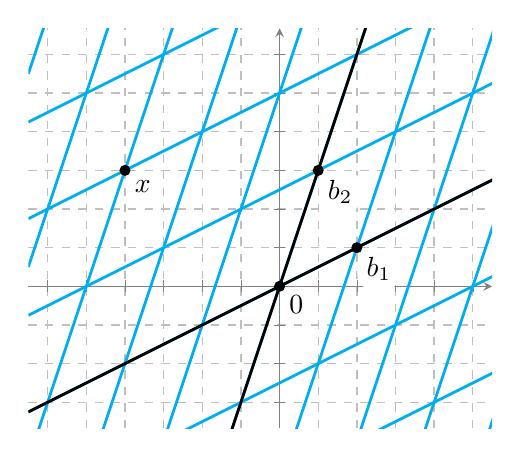
\begin{tikzpicture}[scale=1]
	% Set u and v
	\pgfmathsetmacro{\ux}{2}
	\pgfmathsetmacro{\uy}{1}
	\pgfmathsetmacro{\vx}{1}
	\pgfmathsetmacro{\vy}{3}
	\pgfmathsetmacro{\xcoor}{-4}
	\pgfmathsetmacro{\ycoor}{3}
	% Begin Axis
	\begin{axis}[axis x line=center, axis y line=middle,
	xmin=-6.5, xmax=5.5,
	ymin=-3.5, ymax=6.5,
	xtick={-6,...,5}, ytick={-3,...,7},
	xticklabels={,,}, yticklabels={,,},
	scale only axis, axis equal, height=2in,
	gray,
	grid=major, grid style={line width=.5pt, draw=gray!50, dashed}]
	% Plot alternate coordinate system
	\foreach \yi in {-10,...,10}{
		\addplot[-, cyan, line width=1pt, domain=-6.5:6.5] {(\uy/\ux)*(x-\yi*\vx)+\vy*\yi};
	}
	\foreach \xi in {-10,...,10}{
		\addplot[-, cyan, line width=1pt, domain=-6.5:6.5] {(\vy/\vx)*(x-\xi*\ux)+\uy*\xi};
	}
	\addplot[-, black, line width=1pt, domain=-6.5:6.5] {(\uy/\ux)*x};
	\addplot[-, black, line width=1pt, domain=-6.5:6.5] {(\vy/\vx)*x};
	% Plot vectors
	\fill[black] (0,0) circle (2pt) node[below right, fill=white, rounded corners=0.2cm] {$\vect{0}$};
	\fill[black] (\ux,\uy) circle (2pt) node[below right, fill=white, rounded corners=0.2cm] {$\vect{b}_1$};
	\fill[black] (\vx,\vy) circle (2pt) node[below right, fill=white, rounded corners=0.2cm] {$\vect{b}_2$};
	\fill[black] (\xcoor,\ycoor) circle (2pt) node[below right, fill=white, rounded corners=0.2cm] {$\vect{x}$};
	\end{axis}
	\end{tikzpicture}
	\end{center}
	\end{multicols}
\end{exercise}

\vfill

\begin{boxthm}
	\textbf{Theorem} \\
	If a vector space $H$ has a basis of $n$ vectors, then every basis for $H$ must consist of exactly $n$ vectors.
\end{boxthm}
\vspace{-1em}
\begin{boxdef}
	The \textbf{dimension} of a vector space $H$, denoted $\dim H$, is the number of vectors in a basis for $H$.
\end{boxdef}

\begin{boxme}
	The dimension of $\Nul A$ is the number of free variables in the equation $\Axz$. \\
	The dimension of $\Col A$ is the number of pivot columns in $A$.
\end{boxme}


\newpage

\begin{boxdef}
	The \textbf{rank} of $A$ is the dimension of the column space of $A$.
\end{boxdef}

\begin{boxthm}
	\textbf{Theorem 2.14.}
	\textbf{The Rank Theorem} \\
	The dimension of the column space and the row space of an $m\times n$ matrix $A$ are equal. This common dimension, the rank of $A$, also equals the number of pivot positions in $A$ and satisfies the equation
	\vspace{-1em}
	$$ \rank A + \dim\Nul A = n. $$
\end{boxthm}


\begin{exercise} % 4.5.13 & 15
	Determine the dimensions of the null space and column space for $A$.
	\begin{multicols}{2}
	\begin{enumerate}[(a)]
		\item $$A=\begin{bmatrix}1&-5&-5&3&-6\\0&1&7&-2&2\\0&0&0&-6&-9\\0&0&0&0&1\end{bmatrix}$$
		\vfill
		
		$\boldsymbol{\dim\Nul A=}$ \\[1em]
		$\boldsymbol{\rank A = \dim\Col A=}$

	\end{enumerate}
	\end{multicols}
\end{exercise}
\vfill


\begin{boxthm}
	\textbf{Theorem} \\
	If a subspace $H$ of $\mathbb{R}^n$ has a basis $\B=\vectset[b]{1}{p}$, then any set in $H$ containing more than $p$ vectors must be linearly dependent.
\end{boxthm}
\vspace{-1em}
\begin{boxthm}
	\textbf{Theorem 2.15.}
	\textbf{The Basis Theorem} \\
	Let $H$ be a $p$-dimensional subspace of $\mathbb{R}^n$. Any linearly independent set of vectors of exactly $p$ elements in $H$ is automatically a basis for $H$. Any set of exactly $p$ elements that spans $H$ is automatically a basis for $H$.
\end{boxthm}


\begin{exercise} % 4.5.Custom
	Use the above theorems to answer the questions here.
	\begin{multicols}{2}
		\begin{enumerate}[(a)]
			\item The set of vectors below span $\R^5$.
			$$\left\{
			\begin{bmatrix}1\\2\\1\\0\\1\end{bmatrix},
			\begin{bmatrix}1\\0\\1\\1\\1\end{bmatrix},
			\begin{bmatrix}1\\2\\1\\3\\1\end{bmatrix},
			\begin{bmatrix}1\\2\\3\\1\\1\end{bmatrix},
			\begin{bmatrix}1\\0\\0\\0\\0\end{bmatrix},
			\begin{bmatrix}0\\0\\0\\0\\1\end{bmatrix}
			\right\}$$
			Is this set a basis for $\R^5$? Explain.
			
			\columnbreak
			\item 
			$$\left\{
			\begin{bmatrix}1\\0\\0\end{bmatrix},
			\begin{bmatrix}1\\4\\0\end{bmatrix},
			\begin{bmatrix}1\\2\\1\end{bmatrix}
			\right\}$$
			Is this set a basis for $\R^3$? Explain.
		\end{enumerate}
	\end{multicols}
\end{exercise}
\vfill

\newpage
